\newpage
\section{空気圧人工筋肉}
\subsection{McKibben型空気圧人工筋肉アクチュエータ(MPA)}
MPAはシリコンゴムチューブをナイロンメッシュで覆うことで構成されており(図\ref{fig:MPA}\subref{fig:Structure}),両端に栓をするシンプルな構造である.
これに圧縮した空気を印加することでシリコンゴムチューブが膨張しメッシュによる自身の軸方向への張力が発生するアクチュエータである(図\ref{fig:MPA}\subref{fig:move}).
高出力かつ素材自体も軽量で,物理的柔軟性による高い弾性力を持つという利点があり,筋肉の代用として生物を模したロボットやリハビリなどに用いられる.
しかし図1に示すような従来の直径が数10 mmのMPAは,さらなる高集積化や小動物型や昆虫型などの非常に小型なロボットへの応用を考慮した場合,そのサイズは大きすぎる
%%%%%%%%%%%%%%%%%%%%%%%%%%%%%%%%%%%%%%%%%%%%%%%%%%%%%%%%%
\begin{figure}[b]
    %
    \begin{minipage}{0.49\columnwidth}
      \vspace{4mm}
      \centering
      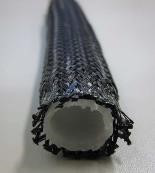
\includegraphics[scale=1]{pic/MPA_kousei.png}
      \vspace{3mm}
      \subcaption{MPA断面図}
      \label{fig:Structure}
    \end{minipage}
    %
    \begin{minipage}{0.49\columnwidth}
      \vspace{25mm}
      \centering
      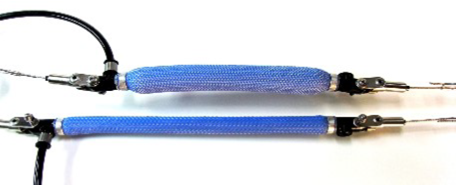
\includegraphics[scale=.8]{pic/MPA_dousa.png}
      \subcaption{MPA外観および動作の様子}
      \label{fig:move}
    \end{minipage}
    %
    \caption{McKibben型空気圧人工筋(MPA)の構成および外観\cite{中西大輔2020}}
    \label{fig:MPA}
  \end{figure}.
  \begin{figure}[!b]
    \centering  % 図全体を中央に配置
    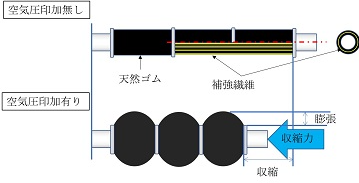
\includegraphics[scale=0.7]{pic/A.PNG}
    \caption{軸方向繊維強化型人工筋肉の仕組み\cite{4}}
  \end{figure}
  
\subsection{軸方向繊維強化型人工筋肉}
本研究で開発する超細径空圧筋のベースとなる,軸方向繊維強化型人工筋肉の動作原理を図1に示す.
この人工筋肉は,ゴムチューブ内に拘束繊維を内包する構造で,拘束繊維とゴムチューブとの摩耗を抑え長寿命を実現する.
空気圧が供給されると,内圧が半径方向にのみ伝達され,軸方向への効率的な収縮を引き起こす.
さらに,チューブに外挿されたリングの数を調整することで,ゴムチューブの膨張を抑制しつつ必要な収縮力を発揮できる\cite{3}.

